\section{Quantities and Units}
\label{sec:Quantities}
%%%%%%%%%%%%%%%%%%%%%%%%%%%%%%%%%%%%%%%%%%%%%%%%%%%%%%%%
\begin{figure}[h!]
\begin{center}
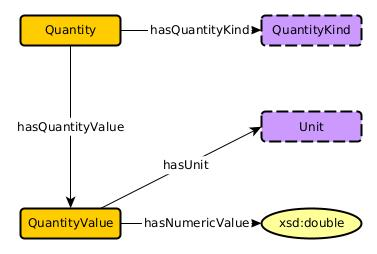
\includegraphics[width=.7\textwidth]{figures/quantity}
\end{center}
\caption{Schema Diagram for Quantities and Units. The visual notation is explained in Chapter \ref{chap:prelims}.}
\label{fig:Quantities}
\end{figure}
\subsection{Summary}
\label{sum:Quantities}
%%%%%%%%%%%%%%%%%%%%%%%%%%%%
This pattern is heavily adapted from QUDT\footnote{\url{http://www.qudt.org/release2/qudt-catalog.html}} and \cite{momtut}. This pattern allows a developer to express a quantity of some stuff. The nature of quantity is rather complex, due to the fact that there are a multitude of dimensions, unit types, and ways to measure quantity. The \textsf{Quantity} class is used to express the nature of the quantity via its \textsf{QuantityKind}. This is intended to be a controlled vocabulary. We direct the reader to QUDT's documentation for further exploration. A \textsf{QuantityValue} expresses the magnitude of the \textsf{Quantity} via an \textsf{xsd:double} and a \textsf{Unit}. Unit is also recommended to be a controlled vocabulary. Both \textsf{hasQuantityKind} and \textsf{hasUnit} are instances of the Explicit Typing Pattern (Section \ref{sec:Explicit}).

%%%%%%%%%%%%%%%%%%%%%%%%%%%%%%%%%%%%%%%%%%%%%%%%%%%%%%%%
\subsection{Axiomatization}
\label{axs:Quantities}
%%%%%%%%%%%%%%%%%%%%%%%%%%%%
\begin{align}
\top &\sqsubseteq \forall \textsf{hasQuantityKind.QuantityKind} \\
\top &\sqsubseteq \forall \textsf{hasQuantityValue.QuantityValue} \\
\top &\sqsubseteq \forall \textsf{hasUnit.Unit} \\
\top &\sqsubseteq \forall \textsf{hasNumericalValue.xsd:double}
\end{align}

%%%%%%%%%%%%%%%%%%%%%%%%%%%%%%%%%%%%%%%%%%%%%%%%%%%%%%%%
\subsection{Explanations}
\label{exp:Quantities}
%%%%%%%%%%%%%%%%%%%%%%%%%%%%
\begin{enumerate}
\item Range: the range of \textsf{hasQuantityKind} is \textsf{QuantityKind}.
\item Range: the range of \textsf{hasQuantityValue} is \textsf{QuantityValue}.
\item Range: the range of \textsf{hasUnit} is \textsf{Unit}.
\item Range: the range of \textsf{hasNumericValue} is \textsf{xsd:double}.
\end{enumerate}

%%%%%%%%%%%%%%%%%%%%%%%%%%%%%%%%%%%%%%%%%%%%%%%%%%%%%%%%
\subsection{Competency Questions}
\label{cqs:Quantities}
%%%%%%%%%%%%%%%%%%%%%%%%%%%%
\begin{enumerate}[CQ1.]
\item How much does an elephant weigh in kilograms?
\item How long is Jupiter from the Sun, at its farthest, in furlongs?
\item How long ago was the Mezazoic Era?
\end{enumerate}

\newpage
%%%%%%%%%%%%%%%%%%%%%%%%%%%%%%%%%%%%%%%%%%%%%%%%%%%%%%%%
% End Section
%%%%%%%%%%%%%%%%%%%%%%%%%%%%%%%%%%%%%%%%%%%%%%%%%%%%%%%%
%%%%%%%%%%%%%%%%%%%%%%%%%%%%%%%%%%%%%%%%%%%%%%%%%%%%%%%%